\documentclass[tikz,border=3pt]{standalone}
\usepackage[T1]{fontenc}
\usepackage{helvet}
\renewcommand{\familydefault}{\sfdefault}
\usetikzlibrary{arrows.meta}
\begin{document}
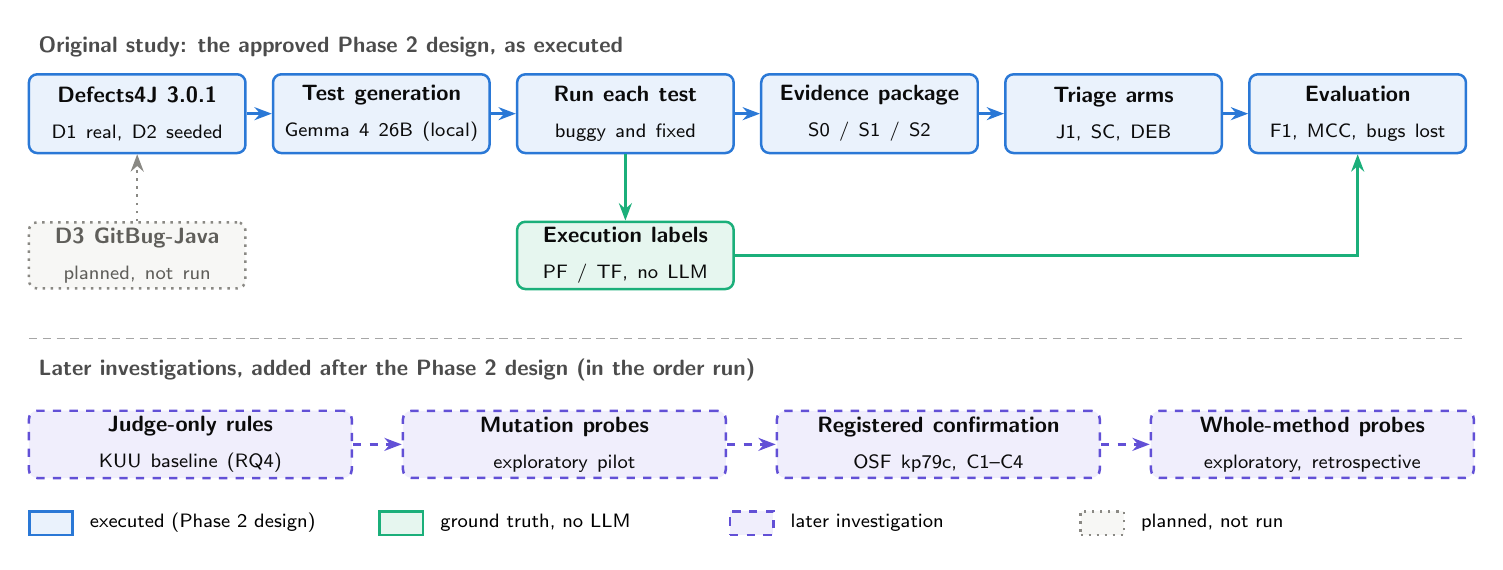
\begin{tikzpicture}[>={Stealth[length=2.2mm]}]
\definecolor{fdone}{HTML}{EAF2FC}\definecolor{bdone}{HTML}{2A78D6}\definecolor{tdone}{HTML}{0B0B0B}
\definecolor{fgt}{HTML}{E6F6EF}\definecolor{bgt}{HTML}{1BAF7A}\definecolor{tgt}{HTML}{0B0B0B}
\definecolor{fext}{HTML}{F0EEFC}\definecolor{bext}{HTML}{6250D6}\definecolor{text}{HTML}{0B0B0B}
\definecolor{fnotrun}{HTML}{F7F7F5}\definecolor{bnotrun}{HTML}{8A8984}\definecolor{tnotrun}{HTML}{5F5E5A}
\node[anchor=west,font=\footnotesize\bfseries,text=black!70] at (0,0.85) {Original study: the approved Phase 2 design, as executed};
\draw[densely dashed,black!35] (0,-2.85) -- (18.25,-2.85);
\node[anchor=west,font=\footnotesize\bfseries,text=black!70] at (0,-3.25) {Later investigations, added after the Phase 2 design (in the order run)};
\node[draw=bdone,fill=fdone,text=tdone,solid,line width=0.9pt,rounded corners=3pt,minimum width=2.75cm,minimum height=1.0cm,text width=2.55cm,align=center,inner sep=2pt,execute at begin node={\hyphenpenalty=10000\relax}] (data) at (1.375,0) {{\footnotesize\bfseries Defects4J 3.0.1}\\[1pt]{\scriptsize D1 real, D2 seeded}};
\node[draw=bdone,fill=fdone,text=tdone,solid,line width=0.9pt,rounded corners=3pt,minimum width=2.75cm,minimum height=1.0cm,text width=2.55cm,align=center,inner sep=2pt,execute at begin node={\hyphenpenalty=10000\relax}] (gen) at (4.475,0) {{\footnotesize\bfseries Test generation}\\[1pt]{\scriptsize Gemma 4 26B (local)}};
\node[draw=bdone,fill=fdone,text=tdone,solid,line width=0.9pt,rounded corners=3pt,minimum width=2.75cm,minimum height=1.0cm,text width=2.55cm,align=center,inner sep=2pt,execute at begin node={\hyphenpenalty=10000\relax}] (run) at (7.575,0) {{\footnotesize\bfseries Run each test}\\[1pt]{\scriptsize buggy and fixed}};
\node[draw=bdone,fill=fdone,text=tdone,solid,line width=0.9pt,rounded corners=3pt,minimum width=2.75cm,minimum height=1.0cm,text width=2.55cm,align=center,inner sep=2pt,execute at begin node={\hyphenpenalty=10000\relax}] (ctx) at (10.675,0) {{\footnotesize\bfseries Evidence package}\\[1pt]{\scriptsize S0 / S1 / S2}};
\node[draw=bdone,fill=fdone,text=tdone,solid,line width=0.9pt,rounded corners=3pt,minimum width=2.75cm,minimum height=1.0cm,text width=2.55cm,align=center,inner sep=2pt,execute at begin node={\hyphenpenalty=10000\relax}] (arms) at (13.775,0) {{\footnotesize\bfseries Triage arms}\\[1pt]{\scriptsize J1, SC, DEB}};
\node[draw=bdone,fill=fdone,text=tdone,solid,line width=0.9pt,rounded corners=3pt,minimum width=2.75cm,minimum height=1.0cm,text width=2.55cm,align=center,inner sep=2pt,execute at begin node={\hyphenpenalty=10000\relax}] (eval) at (16.875,0) {{\footnotesize\bfseries Evaluation}\\[1pt]{\scriptsize F1, MCC, bugs lost}};
\node[draw=bnotrun,fill=fnotrun,text=tnotrun,dotted,line width=0.9pt,rounded corners=3pt,minimum width=2.75cm,minimum height=0.8cm,text width=2.55cm,align=center,inner sep=2pt,execute at begin node={\hyphenpenalty=10000\relax}] (d3) at (1.375,-1.8) {{\footnotesize\bfseries D3 GitBug-Java}\\[1pt]{\scriptsize planned, not run}};
\node[draw=bgt,fill=fgt,text=tgt,solid,line width=0.9pt,rounded corners=3pt,minimum width=2.75cm,minimum height=0.8cm,text width=2.55cm,align=center,inner sep=2pt,execute at begin node={\hyphenpenalty=10000\relax}] (label) at (7.575,-1.8) {{\footnotesize\bfseries Execution labels}\\[1pt]{\scriptsize PF / TF, no LLM}};
\node[draw=bext,fill=fext,text=text,dashed,line width=0.9pt,rounded corners=3pt,minimum width=4.1cm,minimum height=0.85cm,text width=3.8999999999999995cm,align=center,inner sep=2pt,execute at begin node={\hyphenpenalty=10000\relax}] (rules) at (2.05,-4.2) {{\footnotesize\bfseries Judge-only rules}\\[1pt]{\scriptsize KUU baseline (RQ4)}};
\node[draw=bext,fill=fext,text=text,dashed,line width=0.9pt,rounded corners=3pt,minimum width=4.1cm,minimum height=0.85cm,text width=3.8999999999999995cm,align=center,inner sep=2pt,execute at begin node={\hyphenpenalty=10000\relax}] (cfp) at (6.8,-4.2) {{\footnotesize\bfseries Mutation probes}\\[1pt]{\scriptsize exploratory pilot}};
\node[draw=bext,fill=fext,text=text,dashed,line width=0.9pt,rounded corners=3pt,minimum width=4.1cm,minimum height=0.85cm,text width=3.8999999999999995cm,align=center,inner sep=2pt,execute at begin node={\hyphenpenalty=10000\relax}] (conf) at (11.55,-4.2) {{\footnotesize\bfseries Registered confirmation}\\[1pt]{\scriptsize OSF kp79c, C1--C4}};
\node[draw=bext,fill=fext,text=text,dashed,line width=0.9pt,rounded corners=3pt,minimum width=4.1cm,minimum height=0.85cm,text width=3.8999999999999995cm,align=center,inner sep=2pt,execute at begin node={\hyphenpenalty=10000\relax}] (wdp) at (16.3,-4.2) {{\footnotesize\bfseries Whole-method probes}\\[1pt]{\scriptsize exploratory, retrospective}};
\draw[->,draw=bdone,solid,line width=0.9pt] (data.east) -- (gen.west);
\draw[->,draw=bdone,solid,line width=0.9pt] (gen.east) -- (run.west);
\draw[->,draw=bdone,solid,line width=0.9pt] (run.east) -- (ctx.west);
\draw[->,draw=bdone,solid,line width=0.9pt] (ctx.east) -- (arms.west);
\draw[->,draw=bdone,solid,line width=0.9pt] (arms.east) -- (eval.west);
\draw[->,draw=bnotrun,dotted,line width=0.9pt] (d3.north) -- (data.south);
\draw[->,draw=bgt,solid,line width=0.9pt] (run.south) -- (label.north);
\draw[->,draw=bgt,solid,line width=0.9pt] (label.east) -| (eval.south);
\draw[->,draw=bext,dashed,line width=0.9pt] (rules.east) -- (cfp.west);
\draw[->,draw=bext,dashed,line width=0.9pt] (cfp.east) -- (conf.west);
\draw[->,draw=bext,dashed,line width=0.9pt] (conf.east) -- (wdp.west);
\node[draw=bdone,fill=fdone,solid,line width=0.9pt,minimum width=0.55cm,minimum height=0.3cm] at (0.28,-5.2) {};
\node[anchor=west,font=\scriptsize] at (0.65,-5.2) {executed (Phase 2 design)};
\node[draw=bgt,fill=fgt,solid,line width=0.9pt,minimum width=0.55cm,minimum height=0.3cm] at (4.73,-5.2) {};
\node[anchor=west,font=\scriptsize] at (5.1000000000000005,-5.2) {ground truth, no LLM};
\node[draw=bext,fill=fext,dashed,line width=0.9pt,minimum width=0.55cm,minimum height=0.3cm] at (9.18,-5.2) {};
\node[anchor=west,font=\scriptsize] at (9.55,-5.2) {later investigation};
\node[draw=bnotrun,fill=fnotrun,dotted,line width=0.9pt,minimum width=0.55cm,minimum height=0.3cm] at (13.63,-5.2) {};
\node[anchor=west,font=\scriptsize] at (14.000000000000002,-5.2) {planned, not run};
\end{tikzpicture}
\end{document}
